\documentclass[]{book}
\usepackage{lmodern}
\usepackage{amssymb,amsmath}
\usepackage{ifxetex,ifluatex}
\usepackage{fixltx2e} % provides \textsubscript
\ifnum 0\ifxetex 1\fi\ifluatex 1\fi=0 % if pdftex
  \usepackage[T1]{fontenc}
  \usepackage[utf8]{inputenc}
\else % if luatex or xelatex
  \ifxetex
    \usepackage{mathspec}
  \else
    \usepackage{fontspec}
  \fi
  \defaultfontfeatures{Ligatures=TeX,Scale=MatchLowercase}
\fi
% use upquote if available, for straight quotes in verbatim environments
\IfFileExists{upquote.sty}{\usepackage{upquote}}{}
% use microtype if available
\IfFileExists{microtype.sty}{%
\usepackage{microtype}
\UseMicrotypeSet[protrusion]{basicmath} % disable protrusion for tt fonts
}{}
\usepackage[margin=1in]{geometry}
\usepackage{hyperref}
\hypersetup{unicode=true,
            pdftitle={Análise de Dados Amostrais Complexos},
            pdfauthor={Djalma Pessoa e Pedro Nascimento Silva},
            pdfborder={0 0 0},
            breaklinks=true}
\urlstyle{same}  % don't use monospace font for urls
\usepackage{natbib}
\bibliographystyle{apalike}
\usepackage{longtable,booktabs}
\usepackage{graphicx,grffile}
\makeatletter
\def\maxwidth{\ifdim\Gin@nat@width>\linewidth\linewidth\else\Gin@nat@width\fi}
\def\maxheight{\ifdim\Gin@nat@height>\textheight\textheight\else\Gin@nat@height\fi}
\makeatother
% Scale images if necessary, so that they will not overflow the page
% margins by default, and it is still possible to overwrite the defaults
% using explicit options in \includegraphics[width, height, ...]{}
\setkeys{Gin}{width=\maxwidth,height=\maxheight,keepaspectratio}
\IfFileExists{parskip.sty}{%
\usepackage{parskip}
}{% else
\setlength{\parindent}{0pt}
\setlength{\parskip}{6pt plus 2pt minus 1pt}
}
\setlength{\emergencystretch}{3em}  % prevent overfull lines
\providecommand{\tightlist}{%
  \setlength{\itemsep}{0pt}\setlength{\parskip}{0pt}}
\setcounter{secnumdepth}{5}
% Redefines (sub)paragraphs to behave more like sections
\ifx\paragraph\undefined\else
\let\oldparagraph\paragraph
\renewcommand{\paragraph}[1]{\oldparagraph{#1}\mbox{}}
\fi
\ifx\subparagraph\undefined\else
\let\oldsubparagraph\subparagraph
\renewcommand{\subparagraph}[1]{\oldsubparagraph{#1}\mbox{}}
\fi

%%% Use protect on footnotes to avoid problems with footnotes in titles
\let\rmarkdownfootnote\footnote%
\def\footnote{\protect\rmarkdownfootnote}

%%% Change title format to be more compact
\usepackage{titling}

% Create subtitle command for use in maketitle
\newcommand{\subtitle}[1]{
  \posttitle{
    \begin{center}\large#1\end{center}
    }
}

\setlength{\droptitle}{-2em}
  \title{Análise de Dados Amostrais Complexos}
  \pretitle{\vspace{\droptitle}\centering\huge}
  \posttitle{\par}
  \author{Djalma Pessoa e Pedro Nascimento Silva}
  \preauthor{\centering\large\emph}
  \postauthor{\par}
  \predate{\centering\large\emph}
  \postdate{\par}
  \date{2017-11-16}

\usepackage{booktabs}
\usepackage[brazil]{babel}

\usepackage{amsthm}
\newtheorem{theorem}{Teorema}[chapter]
\newtheorem{lemma}{Lema}[chapter]
\theoremstyle{definition}
\newtheorem{definition}{Definição}[chapter]
\newtheorem{corollary}{Corolário}[chapter]
\newtheorem{proposition}{Proposição}[chapter]
\theoremstyle{definition}
\newtheorem{example}{Exemplo}[chapter]
\theoremstyle{definition}
\newtheorem{exercise}{Exercise}[chapter]
\theoremstyle{remark}
\newtheorem*{remark}{Observação}
\newtheorem*{solution}{Solution}
\let\BeginKnitrBlock\begin \let\EndKnitrBlock\end
\begin{document}
\maketitle

{
\setcounter{tocdepth}{1}
\tableofcontents
}
\chapter*{Prefácio}\label{prefacio}
\addcontentsline{toc}{chapter}{Prefácio}

\section*{Agradecimentos}\label{agradecimentos}
\addcontentsline{toc}{section}{Agradecimentos}

\chapter{Introdução}\label{introduc}

\section{Motivação}\label{motivacao}

\section{Objetivos do Livro}\label{objetivos-do-livro}

\section{Laboratório de R do Capítulo 1.}\label{epa}

\section{{[}1{]} 19409 13}\label{section}

\section{\texorpdfstring{{[}1{]} ``serie'' ``ident'' ``codmor''
``v04a01'' ``v04a02''
``v04a03''}{{[}1{]} serie ident codmor v04a01 v04a02 v04a03}}\label{serie-ident-codmor-v04a01-v04a02-v04a03}

\section{\texorpdfstring{{[}7{]} ``estratof'' ``peso1'' ``peso2''
``pesof'' ``nsetor''
``regiao''}{{[}7{]} estratof peso1 peso2 pesof nsetor regiao}}\label{estratof-peso1-peso2-pesof-nsetor-regiao}

\section{\texorpdfstring{{[}13{]}
``v02a08''}{{[}13{]} v02a08}}\label{v02a08}

\section{total SE DEff}\label{total-se-deff}

\section{analf1 1174220 127982
2.0543}\label{analf1-1174220-127982-2.0543}

\section{total SE DEff}\label{total-se-deff-1}

\section{analf2 4792344 318877
3.3237}\label{analf2-4792344-318877-3.3237}

\section{Ratio estimator:
svyratio.survey.design2(\textasciitilde{}analf1,
\textasciitilde{}faixa1,
ppv\_se\_plan)}\label{ratio-estimator-svyratio.survey.design2analf1-faixa1-ppv_se_plan}

\section{Ratios=}\label{ratios}

\section{faixa1}\label{faixa1}

\section{analf1 0.118689}\label{analf1-0.118689}

\section{SEs=}\label{ses}

\section{faixa1}\label{faixa1-1}

\section{analf1 0.01178896}\label{analf1-0.01178896}

\section{Ratio estimator:
svyratio.survey.design2(\textasciitilde{}analf2,
\textasciitilde{}faixa2,
ppv\_se\_plan)}\label{ratio-estimator-svyratio.survey.design2analf2-faixa2-ppv_se_plan}

\section{Ratios=}\label{ratios-1}

\section{faixa2}\label{faixa2}

\section{analf2 0.1086871}\label{analf2-0.1086871}

\section{SEs=}\label{ses-1}

\section{faixa2}\label{faixa2-1}

\section{analf2 0.006732254}\label{analf2-0.006732254}

\section{regiao analf1 se
DEff.analf1}\label{regiao-analf1-se-deff.analf1}

\section{1 1 3512866 352619.5 9.660561}\label{section-1}

\section{2 2 1174220 127982.2 2.054345}\label{section-2}

\section{Laboratório de R do Capítulo 1 -
Extra.}\label{laboratorio-de-r-do-capitulo-1---extra.}

\section{Taxa Erro\_Padrão CV}\label{taxa-erro_padrao-cv}

\section{1 11.80303 0.1174791 0.9953299}\label{section-3}

\section{{[}1{]} 60202 1019}\label{section-4}

\section{diag\_dep}\label{diag_dep}

\section{7.6}\label{section-5}

\section{diag\_dep}\label{diag_dep-1}

\section{diag\_dep 0.2}\label{diag_dep-0.2}

\section{{[}1{]} 7.2 8.1}\label{section-6}

\section{diag\_dep}\label{diag_dep-2}

\section{7.6 7.2 8.1}\label{section-7}

\section{Apêndice: Estimativa do efeito de plano amostral
(EPA)}\label{apendice-estimativa-do-efeito-de-plano-amostral-epa}

\section{analf1}\label{analf1}

\section{analf1 2.054049}\label{analf1-2.054049}

\section{analf2}\label{analf2}

\section{analf2 3.32324}\label{analf2-3.32324}

\section{total SE DEff}\label{total-se-deff-2}

\section{{[}1,{]} 1174220 127982 2.6426}\label{section-8}

\section{total SE DEff}\label{total-se-deff-3}

\section{{[}1,{]} 4792344 318877 4.1667}\label{section-9}

\section{total SE DEff}\label{total-se-deff-4}

\section{I(ifelse(regiao == 2, analf1, 0)) 1174220 127982
2.6426}\label{iifelseregiao-2-analf1-0-1174220-127982-2.6426}

\section{total SE DEff}\label{total-se-deff-5}

\section{I(ifelse(regiao == 2, analf2, 0)) 4792344 318877
4.1667}\label{iifelseregiao-2-analf2-0-4792344-318877-4.1667}

\chapter{Referencial para Inferência}\label{refinf}

\section{Modelagem - Primeiras Ideias}\label{classic}

Com o objetivo de dar uma primeira ideia sobre o assunto a ser tratado
neste livro vamos considerar, numa situação simples, algumas abordagens
alternativas de análise estatística.

\subsection{Abordagem 1 - Modelagem
Clássica}\label{abordagem-1---modelagem-classica}

Seja \(Y\) um vetor \(P \times 1\) de variáveis de pesquisa (ou de
interesse), e sejam \(n\) vetores de observações destas variáveis para
uma amostra de unidades de interesse denotados por \(y_1,\ldots ,y_n\).
Em Inferência Estatística, a abordagem que aqui chamamos de
\texttt{Modelagem\ clássica} considera \(y_1,\ldots ,y_n\) como valores
(realizações) de vetores de variáveis aleatórias \(Y_1,\ldots ,Y_n\).

Podemos formular modelos bastante sofisticados para a distribuição
conjunta destes vetores aleatórios, mas para simplificar a discussão,
vamos inicialmente supor que \(Y_1,\ldots ,Y_n\) são vetores aleatórios
independentes e identicamente distribuídos (IID), com a mesma
distribuição de \(Y\), caracterizada pela função de densidade ou de
frequência \(f(y;\theta)\), onde \(\theta \in \Theta\) é o parâmetro (um
vetor de dimensão \(K \times 1\)) indexador da distribuição \(f\), e
\(\Theta\) é o espaço paramétrico. A partir das observações
\(y_1,\ldots ,y_n\), são feitas inferências a respeito do parâmetro
\(\theta\).

Uma representação gráfica esquemática dessa abordagem é apresentada na
Figura \ref{fig:modclas}, e uma descrição esquemática resumida é
apresentada na Tabela \ref{tab:modelclass}.

\begin{figure}
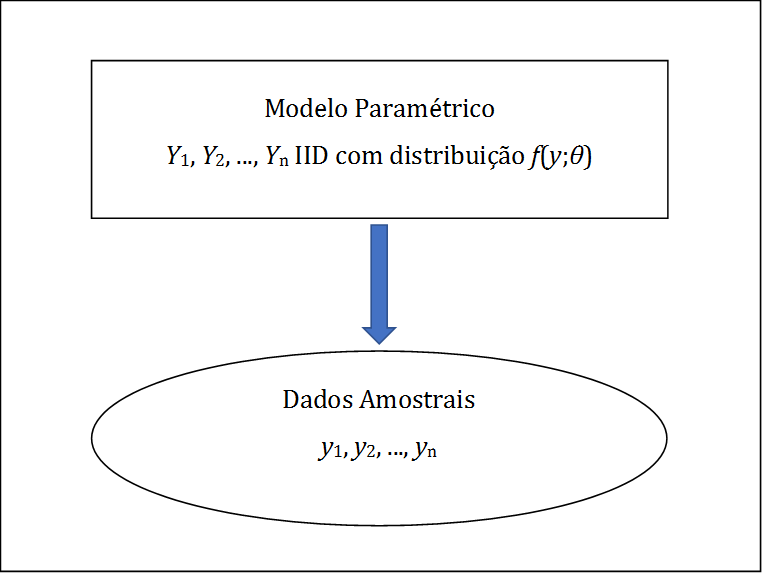
\includegraphics[width=10.6in]{Figuras/Figura2.1} \caption{Modelagem Clássica}\label{fig:modclas}
\end{figure}

\begin{longtable}[]{@{}ll@{}}
\caption{\label{tab:modelclass} Representação esquemática da abordagem
1.}\tabularnewline
\toprule
\begin{minipage}[t]{0.29\columnwidth}\raggedright\strut
Dados Amostrais\strut
\end{minipage} & \begin{minipage}[t]{0.60\columnwidth}\raggedright\strut
\(Y_1=y_1,\ldots, Y_n=y_n\)\strut
\end{minipage}\tabularnewline
\begin{minipage}[t]{0.29\columnwidth}\raggedright\strut
Modelo Paramétrico/ Hipóteses\strut
\end{minipage} & \begin{minipage}[t]{0.60\columnwidth}\raggedright\strut
\(Y_1,\ldots,Y_n\) variáveis aleatórias IID com distribuição
\(f(y,\theta)\), onde \(\theta \in \Theta\)\strut
\end{minipage}\tabularnewline
\begin{minipage}[t]{0.29\columnwidth}\raggedright\strut
Objetivo\strut
\end{minipage} & \begin{minipage}[t]{0.60\columnwidth}\raggedright\strut
Inferir sobre \(\theta\) usando as observações \(y_1, \ldots,y_n\)\strut
\end{minipage}\tabularnewline
\bottomrule
\end{longtable}

Do ponto de vista matemático, o parâmetro \(\theta\) serve para indexar
os elementos da família de distribuições
\(\left\{f\left( y;\theta \right);\theta \in \Theta \right\}\). Na
prática, as questões relevantes da pesquisa são traduzidas em termos de
perguntas sobre o valor ou região a que pertence o parâmetro \(\theta\),
e a inferência sobre \(\theta\) a partir dos dados ajuda a responder
tais questões. Esta abordagem é útil em estudos analíticos tais como,
por exemplo, na investigação da natureza da associação entre variáveis
(modelos de regressão linear ou logística, modelos log-lineares, etc.).
Vários exemplos discutidos ao longo dos Capítulos \ref{modreg},
\ref{testqualajust} e \ref{testetab2} ilustram situações deste tipo. No
Capítulo \ref{estimacao-de-densidades} o foco vai ser a estimação não
paramétrica da forma da função \(f(y;\theta)\).

Investigando a existência de diferenciais de salários por sexo e raça

Uma questão de grande interesse para o debate sobre a existência de
desigualdades numa sociedade diz respeito à possível existência de
diferenciais de salários entre pessoas de sexo e raça distintos, após
controlar por características do trabalhador tais como escolaridade,
ocupação e experiência, e da firma, tais como tamanho, setor de
atividade e outras. \citep{Rodrigues} examinou este problema empregando
modelos de regressão para explicar o logaritmo do salário hora dos
trabalhadores empregados, ajustados a dados obtidos através da Pesquisa
sobre Padrões de Vida do IBGE, e tomando como variáveis explicativas
características do trabalhador, do posto de trabalho e da empresa. A
autora concluiu que não se pode rejeitar a hipótese de existência de
discriminação racial e de sexo no mercado de trabalho, pois
trabalhadores igualmente produtivos inseridos em trabalhos de
características similares apresentavam diferenciais de salários com base
em atributos não produtivos, como o sexo, a raça, e o estado civil, por
exemplo. Tais conclusões foram obtidas mediante testes de hipóteses
sobre valores dos parâmetros do modelo ajustado.

\subsection{Abordagem 2 - Amostragem
Probabilística}\label{abordagem-2---amostragem-probabilistica}

A abordagem adotada pelos praticantes de amostragem (amostristas)
considera uma população finita \(U=\{1,\ldots ,N\}\), da qual é
selecionada uma amostra \(a=\left\{ i_{1},\ldots ,i_{n}\right\}\),
segundo um plano amostral caracterizado por \(p\left( a\right)\),
probabilidade de ser selecionada a amostra \(a\), suposta calculável
para todas as possíveis amostras. Os valores \(y_{1},\ldots ,y_{N}\) das
variáveis de interesse \(Y\) na população finita são considerados fixos,
porém desconhecidos. Sem perda de generalidade, podemos reindexar a
população de tal forma que a amostra observada seja formada pelos
índices \(s=\{1,\ldots,n\}\) \textbar{}

A partir dos valores observados na amostra, denotados por
\(y_{i_{1}},\ldots,y_{i_{n}}\), são feitas inferências a respeito de
funções dos valores populacionais, digamos
\(g\left( y_{1},\ldots ,y_{N}\right)\). Os valores de tais funções são
quantidades descritivas populacionais (QDPs), também denominadas
\texttt{parâmetros\ da\ população\ finita} pelos amostristas. Em geral,
o objetivo desta abordagem é fazer estudos descritivos utilizando
funções \(g\) particulares, tais como totais
\(g\left( y_{1},\ldots ,y_{N}\right) =\sum_{i=1}^{N}y_{i}\) , médias
\(g\left( y_{1},\ldots ,y_{N}\right) =N^{-1}\sum_{i=1}^{N}y_{i}\),
proporções, razões, etc. Uma descrição esquemática resumida dessa
abordagem é apresentada no Tabela \ref{tab:modelamo}, e uma
representação gráfica resumida na Figura \ref{fig:modamo}.

\begin{figure}
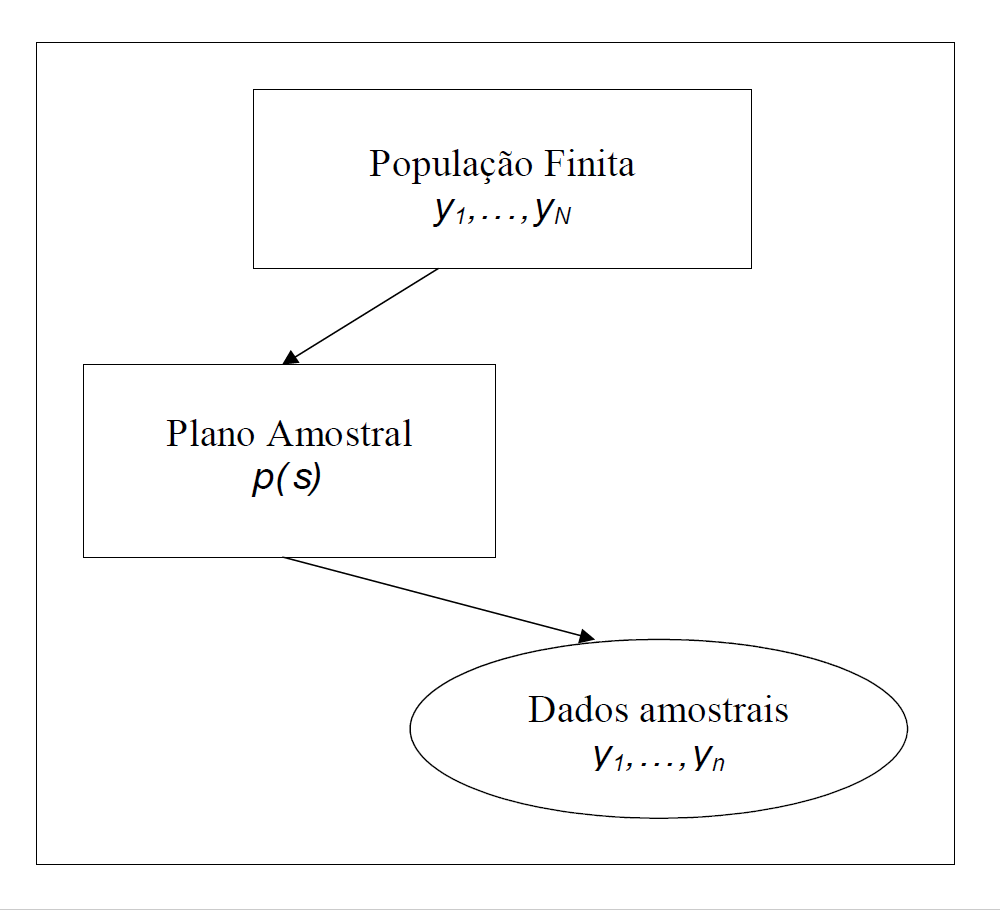
\includegraphics[width=13.89in]{Figuras/fig22} \caption{Amostragem Probabilística}\label{fig:modamo}
\end{figure}

\begin{longtable}[]{@{}ll@{}}
\caption{\label{tab:modelamo} Representação esquemática da abordagem
2.}\tabularnewline
\toprule
\begin{minipage}[t]{0.29\columnwidth}\raggedright\strut
Dados Amostrais\strut
\end{minipage} & \begin{minipage}[t]{0.60\columnwidth}\raggedright\strut
\(Y_1=y_1,\ldots, Y_n=y_n\)\strut
\end{minipage}\tabularnewline
\begin{minipage}[t]{0.29\columnwidth}\raggedright\strut
Hipóteses/Modelo Hipóteses\strut
\end{minipage} & \begin{minipage}[t]{0.60\columnwidth}\raggedright\strut
extraídos de \(y_1,\ldots,y_N\) segundo \(p(s)\)\strut
\end{minipage}\tabularnewline
\begin{minipage}[t]{0.29\columnwidth}\raggedright\strut
Objetivo\strut
\end{minipage} & \begin{minipage}[t]{0.60\columnwidth}\raggedright\strut
Inferir sobre funções \(g(y_1, \ldots, y_N)\) usando
\(y_1, \ldots,y_n\)\strut
\end{minipage}\tabularnewline
\bottomrule
\end{longtable}

Investigando a existência de diferenciais de salários por sexo e raça

Ainda no contexto do exemplo da investigação da existência de
diferenciais de salários por sexo e raça, os dados da Pesquisa sobre
Padrões de Vida do IBGE podem ser utilizados para obter uma tabela
cruzada tendo como entradas de linha o sexo dos trabalhadores, e como
entrada das colunas um indicador de trabalhadores de raça / cor =
branco, sendo as celas da tabela utilizadas para apresentar estimativas
dos valores médios dos salários dos trabalhadores nas várias classes
definidas pelos valores dos indicadores de linha e coluna. Tabelas como
esta são habitualmente produzidas como resultado da realização de
pesquisas amostrais pelas agências oficiais de estatísticas no Brasil e
em muitos outros países. Embora capazes de revelar diferenças nos
salários médios de trabalhadores de sexo e raça distintos, tais tabelas
são insuficientes para investigar a questão da discriminação de gênero
ou raça no mercado de trabalho, pois tais diferenças de salários médios
poderiam ser explicadas por diferenças de características dos
trabalhadores tais como escolaridade, que poderiam ter origem fora do
mercado de trabalho. Por outro lado, ilustram bem os alvos de inferência
freqüentemente definidos para pesquisas amostrais de populações finitas.
Aqui o que se busca estimar é o valor médio de uma característica de
interesse (no caso, o salário) para a população finita de onde foi
extraída a amostra disponível para análise. Apesar de úteis, tais
estimativas representam apenas medidas descritivas da população alvo.

\subsection{Discussão das Abordagens 1 e
2}\label{discussao-das-abordagens-1-e-2}

A primeira abordagem (Modelagem Clássica), nos termos descritos, foi
proposta como modelo para medidas na Física e Astronomia, onde em geral
o pesquisador tem relativo controle sobre os experimentos, e onde faz
sentido falar em replicação ou repetição do experimento. Neste contexto,
o conceito de aleatoriedade é geralmente introduzido para modelar os
erros (não controláveis) no processo de medição.

A segunda abordagem (Amostragem Probabilística) é utilizada
principalmente no contexto de estudos sócio-econômicos, para
levantamento de dados por agências governamentais produtoras de
informações estatísticas. Nesta abordagem, a aleatoriedade é introduzida
no processo pelo pesquisador para obtenção dos dados, através do
planejamento amostral \(p(a)\) utilizado \citep{Neyman} e as
distribuições das estatísticas de interesse são derivadas a partir dessa
\texttt{distribuição\ de\ aleatorização}. Tais planos amostrais podem
ser complexos, gerando observações com as características i) a iv) do
Capítulo \ref{introduc}. Os dados obtidos são utilizados principalmente
para descrição da população finita, sendo calculadas estimativas de
totais, médias, razões, etc. Sob essa abordagem, os pontos i) a iv) do
Capítulo \ref{introduc} são devidamente considerados tanto na estimação
de parâmetros descritivos desses tipos, como também na estimação de
variâncias dos estimadores.

A abordagem de amostragem probabilística é essencialmente
não-paramétrica, pois não supõe uma distribuição paramétrica particular
para as observações da amostra. Por outro lado, essa abordagem tem a
desvantagem de fazer inferências restritas à particular população finita
considerada.

Apesar dessa abordagem ter sido inicialmente concebida e aplicada para
problemas de inferência descritiva sobre populações finitas, é cada vez
mais comum, porém, a utilização de dados obtidos através de pesquisas
amostrais complexas para fins analíticos, com a aplicação de métodos de
análise desenvolvidos e apropriados para a \texttt{abordagem\ 1}.

Diante do exposto, podemos considerar algumas questões de interesse.

\begin{itemize}
\item
  É adequado aplicar métodos de análise da \texttt{abordagem\ 1},
  concebidos para observações IID, aos dados obtidos através de
  pesquisas amostrais complexas?
\item
  Em caso negativo, seria possível corrigir estes métodos, tornando-os
  aplicáveis para tratar dados amostrais complexos?
\item
  Ou seria mais adequado fazer uso analítico dos dados dentro da
  \texttt{abordagem\ 2}? E neste caso, como fazer isto, visto que nesta
  abordagem não é especificado um modelo para a distribuição das
  variáveis de pesquisa \texttt{na\ população}?
\end{itemize}

Além destas, também é de interesse a questão da robustez da modelagem,
traduzida nas seguintes perguntas.

\begin{itemize}
\tightlist
\item
  O que acontece quando o modelo adotado na \texttt{abordagem\ 1} não é
  verdadeiro?
\item
  Neste caso, qual a interpretação do parâmetro na
  \texttt{abordagem\ 1}?
\item
  Ainda neste caso, as quantidades descritivas populacionais da
  \texttt{abordagem\ 2} poderiam ter alguma utilidade ou interpretação?
\end{itemize}

O objeto deste livro é exatamente discutir respostas para as questões
aqui enumeradas. Para isso, vamos considerar uma abordagem que propõe um
modelo parametrizado como na \texttt{abordagem\ 1}, e além disso
incorpora na análise os pontos i) a iii) do Capítulo \ref{introduc}
mediante aproveitamento da estrutura do planejamento amostral como na
\texttt{abordagem\ 2}.

\subsection{Abordagem 3 - Modelagem de
Superpopulação}\label{modelsuperpop}

Nesta abordagem, os valores \(y_{1},\ldots ,y_{N}\) das variáveis de
interesse \(Y\) na população finita são considerados observações ou
realizações dos vetores aleatórios \(Y_{1},\ldots ,Y_{N}\), supostos IID
com distribuição \(f(y;\theta)\), onde \(\theta \in \Theta\). Este
modelo é denominado \texttt{Modelo\ de\ Superpopulação}. Note que, em
contraste com o que se faz na \texttt{abordagem\ 1}, o modelo
probabilístico aqui é especificado para descrever o mecanismo aleatório
que gera \texttt{a\ população}, não \texttt{a\ amostra}, muito embora na
maioria das aplicações práticas a população não será jamais observada
por inteiro. Não obstante, ao formular modelos para a população, nossas
perguntas e respostas descritas em termos de valores ou regiões para o
parâmetro \(\theta\) passam a se referir à população de interesse ou
populações similares, quer existam ao mesmo tempo, quer se refiram a
estados futuros (ou passados) da mesma população.

Utilizando um plano amostral definido por \(p(a)\), obtemos os valores
das variáveis de pesquisa na amostra \(y_{i_1},\ldots ,y_{i_n}\). A
partir de \(y_{i_1},\ldots ,y_{i_n}\) (em geral não considerados como
observações de vetores aleatórios IID) queremos fazer inferências sobre
o parâmetro \(\theta\), considerando os pontos i) a iii) do Capítulo 1.
Veja uma representação gráfica resumida desta abordagem na Figura
\ref{fig:modsup}.

\begin{figure}
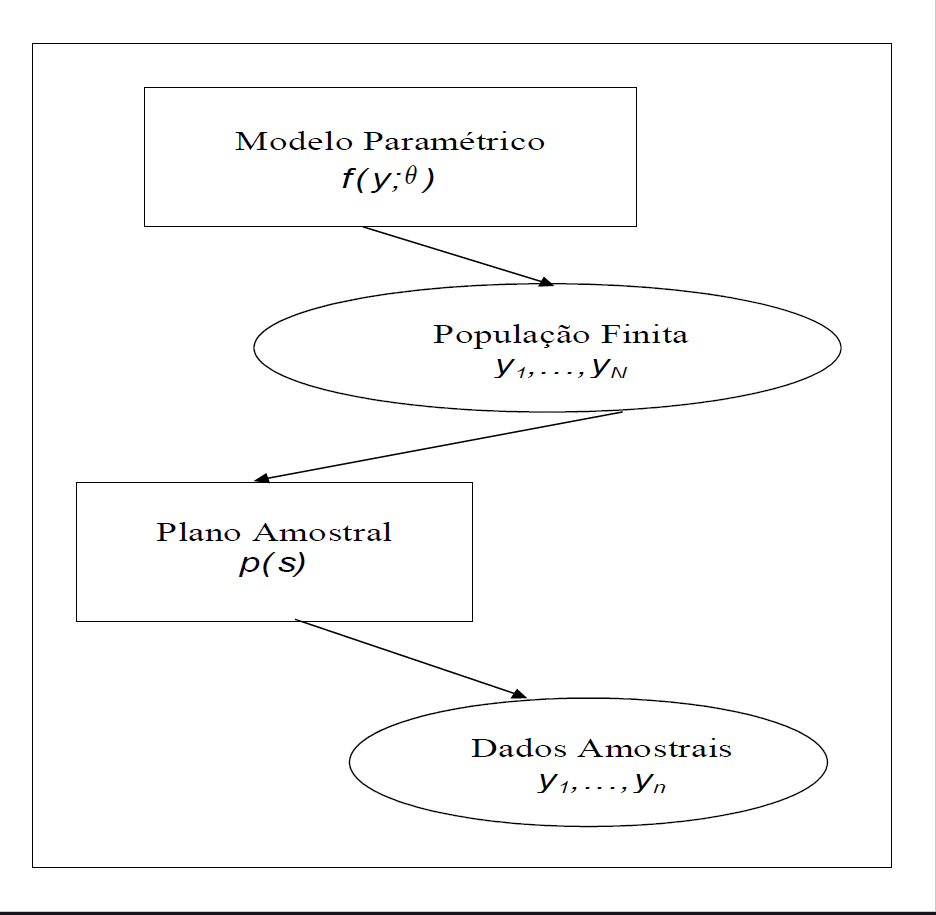
\includegraphics[width=13in]{Figuras/fig23} \caption{Modelagem de Superpopulação}\label{fig:modsup}
\end{figure}

Adotando o modelo de superpopulação e considerando métodos usuais
disponíveis na \texttt{abordagem\ 1}, podemos utilizar funções de
\(y_{1},\ldots ,y_{N}\) , digamos \(g( y_{1},\ldots ,y_{N})\), para
fazer inferências sobre \(\theta\). Desta forma, definimos estatísticas
\(\left( y_{1},\ldots ,y_{N}\right)\) (no sentido da
\texttt{abordagem\ 1}) que são quantidades descritivas populacionais
(parâmetros populacionais no contexto da \texttt{abordagem\ 2}), que
passam a ser os novos parâmetros-alvo. O passo seguinte é utilizar
métodos disponíveis na \texttt{abordagem\ 2} para fazer inferência sobre
\(g\left( y_{1},\ldots ,y_{N}\right)\) baseada em
\(y_{i_1},\ldots ,y_{i_n}\). Note que não é possível basear a inferência
nos valores populacionais \(y_{1},\ldots ,y_{N}\), já que estes não são
conhecidos ou observados. Este último passo adiciona a informação sobre
o plano amostral utilizado, contida em \(p(s)\), à informação estrutural
contida no modelo
\(\left\{ f\left( y;\theta \right) ;\theta \in \Theta\right\}\). Uma
representação esquemática dessa abordagem é apresentada no Tabela
\ref{tab:modelsuperpop}.

\begin{longtable}[]{@{}ll@{}}
\caption{\label{tab:modelsuperpop} Representação esquemática da abordagem
3.}\tabularnewline
\toprule
\begin{minipage}[t]{0.29\columnwidth}\raggedright\strut
Dados Amostrais\strut
\end{minipage} & \begin{minipage}[t]{0.60\columnwidth}\raggedright\strut
\(Y_1=y_1,\ldots, Y_n=y_n\)\strut
\end{minipage}\tabularnewline
\begin{minipage}[t]{0.29\columnwidth}\raggedright\strut
População e esquema de seleção\strut
\end{minipage} & \begin{minipage}[t]{0.60\columnwidth}\raggedright\strut
Extraídos de \(y_1,\dots,y_n\) segundo \(p(s)\)\strut
\end{minipage}\tabularnewline
\begin{minipage}[t]{0.29\columnwidth}\raggedright\strut
Modelo para poulação\strut
\end{minipage} & \begin{minipage}[t]{0.60\columnwidth}\raggedright\strut
\(Y_1,\dots,Y_N\) variáveis aleatórias IID com distribuição
\(f(y,\theta)\), onde \(\theta \in \Theta\)\strut
\end{minipage}\tabularnewline
\begin{minipage}[t]{0.29\columnwidth}\raggedright\strut
Parâmetro-alvo\strut
\end{minipage} & \begin{minipage}[t]{0.60\columnwidth}\raggedright\strut
associar
\(\theta \longleftrightarrow g\left(Y_{1},\ldots Y_{N}\right)\)\strut
\end{minipage}\tabularnewline
\begin{minipage}[t]{0.29\columnwidth}\raggedright\strut
Objetivo\strut
\end{minipage} & \begin{minipage}[t]{0.60\columnwidth}\raggedright\strut
Inferir sobre \(g\left( Y_{1},\ldots Y_{N}\right)\) partir de
\(y_{i_1},\ldots ,y_{i_n}\) usando \(p\left( s\right)\)\strut
\end{minipage}\tabularnewline
\bottomrule
\end{longtable}

A descrição da abordagem adotada neste livro foi apresentada de maneira
propositadamente simplificada e vaga nesta seção, mas será aprofundada
ao longo do texto. Admitiremos que o leitor esteja familiarizado com a
\texttt{abordagem\ 1} e com as noções básicas da \texttt{abordagem\ 2}.
A título de recordação, serão apresentados no Capítulo \ref{planamo}
alguns resultados básicos da Teoria de Amostragem. A ênfase do texto,
porém, será na apresentação da \texttt{abordagem\ 3}, sendo para isto
apresentados os elementos indispensáveis das
\texttt{abordagens\ 1\ e\ 2}.

Ao construir e ajustar modelos a partir de dados de pesquisas amostrais
\texttt{complexas}, tais como as executadas pelo IBGE, o usuário precisa
incorporar as informações sobre pesos e planos amostrais utilizados. Em
geral, ao publicar os resultados das pesquisas, os pesos são
considerados, sendo possível produzir estimativas pontuais
\texttt{corretas} utilizando os pacotes tradicionais. Por outro lado,
para construir intervalos de confiança e testar hipóteses sobre
parâmetros de modelos, seria preciso o conhecimento das estimativas de
variâncias e covariâncias das estimativas, obtidas a partir do plano
amostral utilizado. Mesmo conhecendo o plano amostral, geralmente não é
simples incorporar pesos e plano amostral na análise sem o uso de
pacotes especializados, ou de rotinas específicas já agora disponíveis
em alguns dos pacotes mais comumente utilizados (por exemplo, SAS,
Stata, SPSS, ou R entre outros). Tais pacotes especializados ou rotinas
específicas utilizam na maioria métodos aproximados para estimar
matrizes de covariância, tais como os de Máxima Pseudo-Verossimilhança e
de Linearização, que serão descritos mais adiante.

Em outras palavras, o uso dos pacotes usuais para analisar dados
produzidos por pesquisas com planos amostrais complexos, tal como o uso
de muitos remédios, pode ter contra-indicações. Cabe ao usuário
\texttt{ler\ a\ bula} e identificar situações em que o uso de tais
pacotes pode ser inadequado, e buscar opções de rotinas específicas ou
de pacotes especializados capazes de incorporar adequadamente a
estrutura do plano amostral nas análises. Ao longo deste livro faremos
uso intensivo da library \texttt{survey} disponível no R, mas o leitor
encontrará funcionalidade semelhante em vários outros pacotes. Nossa
escolha se deveu a dois fatores principais: primeiro ao fato do pacote R
ser aberto, livre e gratuito, dispensando o usuário de custos de
licenciamento, bem como possibilitando aos interessados o acesso ao
código fonte e a capacidade de modificar as rotinas de análise, caso
necessário. O segundo fator é de natureza mais técnica, porém
transitória. No presente momento, a library \texttt{survey} é a coleção
de rotinas mais completa e genérica para análise de dados amostrais
complexos existente, dispondo de rotinas capazes de ajustar os modelos
usuais mas também de ajustar modelos não convencionais mediante
maximização de verossimilhanças especificadas pelo usuário. Sabemos,
entretanto, que muitos usuários habituados à facilidade de uso de
pacotes com interfaces gráficas do tipo \texttt{aponte\ e\ clique} terão
dificuldade adicional de adaptar-se à linguagem de comandos utilizada
pelo pacote R, mas acreditamos que os benefícios do aprendizado desta
nova ferramenta compensam largamente os custos adicionais do
aprendizado.

\section{Fontes de Variação}\label{fontes-de-variacao}

Esta seção estabelece um referencial para inferência em pesquisas
amostrais que será usado no restante deste texto. \citep{cassel} sugerem
que um referencial para inferência poderia usar três fontes de
aleatoriedade (incerteza, variação), incluindo:

\begin{enumerate}
\def\labelenumi{\arabic{enumi}.}
\item
  \texttt{modelo\ de\ superpopulação}, que descreve o processo
  subjacente que por hipótese gera as medidas verdadeiras de qualquer
  unidade da população considerada;
\item
  \texttt{processo\ de\ medição}, que diz respeito aos instrumentos e
  métodos usados para obter as medidas de qualquer unidade da população;
\item
  \texttt{planejamento\ amostral}, que estabelece o mecanismo pelo qual
  unidades da população são selecionadas para participar da pesquisa por
  amostra.
\end{enumerate}

Uma quarta fonte de incerteza que precisa ser acrescentada às anteriores
é o

\begin{enumerate}
\def\labelenumi{\arabic{enumi}.}
\setcounter{enumi}{3}
\tightlist
\item
  \texttt{mecanismo\ de\ resposta}, ou seja, o mecanismo que controla se
  valores de medições de unidades selecionadas são disponibilizados ou
  não.
\end{enumerate}

Para concentrar o foco nas questões de maior interesse deste texto, as
fontes (2) e (4) não serão consideradas no referencial adotado para a
maior parte dos capítulos. Para o tratamento das dificuldades causadas
por não resposta, a fonte (4) será considerada no capítulo onze. Assim
sendo, exceto onde explicitamente indicado, de agora em diante
admitiremos que não há erros de medição, implicando que os valores
observados de quaisquer variáveis de interesse serão considerados
valores corretos ou verdadeiros. Admitiremos ainda que há resposta
completa, implicando que os valores de quaisquer variáveis de interesse
estão disponíveis para todos os elementos da amostra selecionada depois
que a pesquisa foi realizada. Hipóteses semelhantes são adotadas, por
exemplo, em \citep{Mont87}.

Portanto, o referencial aqui adotado considera apenas duas fontes
alternativas de variação: o modelo de superpopulação (1) e o plano
amostral (3). Estas fontes alternativas de variação, descritas nesta
seção apenas de forma esquemática, são discutidas com maiores detalhes a
seguir.

A fonte de variação (1) será considerada porque usos analíticos das
pesquisas são amplamente discutidos neste texto, os quais só têm sentido
quando é especificado um modelo estocástico para o processo subjacente
que gera as medidas na população. A fonte de variação (3) será
considerada porque a atenção será focalizada na análise de dados obtidos
através de pesquisas amostrais `complexas. Aqui a discussão se
restringirá a planos amostrais aleatorizados ou de amostragem
probabilística, não sendo considerados métodos intencionais ou outros
métodos não-aleatórios de seleção de amostras.

\section{Modelos de Superpopulação}\label{modelos-de-superpopulacao}

Seja \(\{1,...,N\}\) um conjunto de rótulos que identificam univocamente
os \(N\) elementos distintos de uma população-alvo finita \(U\). Sem
perda de generalidade tomaremos \(U=\{1,...,N\}\). Uma pesquisa cobrindo
\(n\) elementos distintos numa amostra \(a\),
\(a=\{i_{1},...,i_{n}\}\subset U\), é realizada para medir os valores de
\(P\) variáveis de interesse da pesquisa, doravante denominadas
simplesmente variáveis da pesquisa.

Denote por \(\mathbf{y}_i=(y_{i1},...,y_{iP})^{\prime }\) o vetor
\(P\times 1\) de valores das variáveis da pesquisa e por
\(\mathbf{x}_{i}=(x_{i1},...,x_{iQ})^{\prime }\) o vetor \(Q\times 1\)
de variáveis auxiliares da i-ésima unidade da população,
respectivamente, para \(i=1,...,N\). Aqui as variáveis auxiliares são
consideradas como variáveis contendo a informação requerida para o
planejamento amostral e a estimação a partir da amostra, como se
discutirá com mais detalhes adiante. Denote por \(\mathbf{y}_{U}\) a
matriz \(N \times P\) formada empilhando os vetores transpostos das
observações correspondentes a todas as unidades da população, e por
\(\mathbf{Y}_{U}\) a correspondente matriz de vetores aleatórios
geradores das observações na população.

Quando se supõe que \(\mathbf{y}_1 ,\ldots, \mathbf{y}_N\) são a
realização conjunta de vetores aleatórios
\(\mathbf{Y}_1 ,\ldots, \mathbf{Y}_N\), a distribuição conjunta de
probabilidade de \(\mathbf{Y}_1 ,\ldots, \mathbf{Y}_N\) é um modelo
(marginal) de superpopulação, que doravante denotaremos simplesmente por
\(f(\mathbf{y}_U;\theta)\), ou de forma abreviada, por \(M\) para
indicar que se trata do modelo \texttt{marginal} de superpopulação.
Esperanças e variâncias definidas com respeito à distribuição do modelo
marginal \(M\) serão denotadas \(E_M\) e \(V_M\) respectivamente.

Analogamente, \(\mathbf{x}_1 ,\ldots, \mathbf{x}_N\) pode ser
considerada uma realização conjunta de vetores aleatórios
\(\mathbf{X}_1 ,\ldots, \mathbf{X}_N\). As matrizes \(N \times Q\)
formadas empilhando os vetores transpostos das observações das variáveis
auxiliares correspondentes a todas as unidades da população,
\(\mathbf{x}_{U}\), e a correspondente matriz \(\mathbf{X}_{U}\) de
vetores aleatórios geradores das variáveis auxiliares na população são
definidas de forma análoga às matrizes \(\mathbf{y}_{U}\) e
\(\mathbf{Y}_{U}\).

O referencial aqui adotado permite a especificação da distribuição
conjunta combinada das variáveis da pesquisa e das variáveis auxiliares.
Representando por
\(f( \mathbf{y}_U ,\ldots, \mathbf{x}_U ; \mathbf{\eta} )\) a função de
densidade de probabilidade de \(( \mathbf{Y}_U , \mathbf{X}_U )\), onde
\(\mathbf{\eta}\) é um vetor de parâmetros.

Um tipo importante de modelo de superpopulação é obtido quando os
vetores aleatórios correspondentes às observações de elementos
diferentes da população são supostos independentes e identicamente
distribuídos (IID). Neste caso, o modelo de superpopulação pode ser
escrito como:

\begin{eqnarray}
f \left( \mathbf{y}_U , \mathbf{x}_U ; \mathbf{\eta} \right) 
&=&\prod_{i\in U} f\left(\mathbf{y}_i , \mathbf{x}_i ; \mathbf{\eta} \right) \label{eq:ref1} \\
&=&\prod_{i\in U} f\left( \mathbf{y}_i \mathbf{|x}_i ; \mathbf{\lambda} \right) 
f\left( \mathbf{x}_i ; \mathbf{\phi} \right) \label{eq:ref2}
\end{eqnarray}

onde~\(\mathbf{\lambda}\) e \(\mathbf{\phi}\) são vetores de parâmetros.

Sob \eqref{eq:ref2}, o modelo marginal correspondente das variáveis da
pesquisa seria obtido integrando nas variáveis auxiliares:

\begin{equation}
f(\mathbf{y}_U ; \mathbf{\theta}) = f(\mathbf{y}_1 ,\ldots ,\mathbf{y}_N ; \mathbf{\theta}) = \prod_{i\in U} \int f\left( \mathbf{y}_i \mathbf{|x}_i ; \mathbf{\lambda} \right) f\left( \mathbf{x}_i ; \mathbf{\phi} \right) \mathbf{dx}_i = \prod_{i\in U} f\left( \mathbf{y}_i ; \mathbf{\theta} \right) \label{eq:ref3}
\end{equation}

onde
\(f\left( \mathbf{y}_i ; \mathbf{\theta} \right) = \int f\left( \mathbf{y}_i | \mathbf{x}_i ; \mathbf{\lambda} \right) f\left( \mathbf{x}_i ; \mathbf{\phi} \right) \mathbf{dx}_i\)
e
\(\mathbf{\theta =} h\left( \mathbf{\lambda} , \mathbf{\phi} \right)\).

Outro tipo especial de modelo de superpopulação é o modelo de população
fixa, que supõe que os valores numa população finita são fixos mas
desconhecidos. Este modelo pode ser descrito por

\begin{equation}
P\left[ \left( \mathbf{Y}_U , \mathbf{X}_U \right) = \left( \mathbf{y}_U , \mathbf{x}_U \right) \right] = 1 \label{eq:ref4}
\end{equation}

ou seja, uma distribuição degenerada é especificada para
\(\left(\mathbf{Y}_U , \mathbf{X}_U \right)\).

Este modelo foi considerado em \citep{cassel}, que o chamaram de
\texttt{abordagem\ de\ população\ fixa} e afirmaram ser esta a abordagem
subjacente ao desenvolvimento da teoria de amostragem encontrada nos
livros clássicos tais como \citep{cochran} e outros. Aqui esta abordagem
é chamada de abordagem baseada no planejamento amostral ou
\texttt{abordagem\ de\ aleatorização}, pois neste caso a única fonte de
variação (aleatoriedade) é proveniente do planejamento amostral. Em
geral, a distribuição conjunta de
\(\left( \mathbf{Y}_U , \mathbf{X}_U \right)\) não precisa ser
degenerada como em \eqref{eq:ref4}, embora o referencial aqui adotado seja
suficientemente geral para permitir considerar esta possibilidade.

Se todos os elementos fossem pesquisados (ou seja, se fosse executado um
censo), os dados observados seriam
\((\mathbf{y}_1 , \mathbf{x}_1) ,\ldots, (\mathbf{y}_N , \mathbf{x}_N)\).
Sob a hipótese de resposta completa, a única fonte de incerteza seria
devida ao fato de que
\((\mathbf{y}_1 , \mathbf{x}_1) ,\ldots, (\mathbf{y}_N , \mathbf{x}_N)\)
é uma realização de
\(\left( \mathbf{Y}_1 , \mathbf{X}_1 \right) ,\ldots, \left( \mathbf{Y}_N , \mathbf{X}_N \right)\).
Os dados observados poderiam então ser usados para fazer inferências
sobre \(\mathbf{\eta}, \mathbf{\phi},\mathbf{\lambda}\) ou
\(\mathbf{\theta}\) usando procedimentos padrões.

Inferência sobre quaisquer dos parâmetros
\(\mathbf{\eta},\mathbf{\phi},\mathbf{\lambda}\) ou \(\mathbf{\theta}\)
do modelo de superpopulação é chamada \texttt{inferência\ analítica}.
Este tipo de inferência só faz sentido quando o modelo de superpopulação
não é degenerado como em \eqref{eq:ref4}. Usualmente seu objetivo é
explicar a relação entre variáveis não apenas para a população finita
sob análise, mas também para outras populações que poderiam ter sido
geradas pelo modelo de superpopulação adotado. Exemplos de inferência
analítica serão discutidos ao longo deste livro.

Se o objetivo da inferência é estimar quantidades que fazem sentido
somente para a população finita sob análise, tais como funções
\(g\left( \mathbf{y}_1 ,\ldots, \mathbf{y}_N \right)\) dos valores das
variáveis da pesquisa, o modelo de superpopulação não é estritamente
necessário, embora possa ser útil. Inferência para tais quantidades,
chamadas parâmetros da população finita ou quantidades descritivas
populacionais (QDPs), é chamada \texttt{inferência\ descritiva}.

\section{Planejamento Amostral}\label{planamo}

Embora censos sejam algumas vezes realizados para coletar dados sobre
certas populações, a vasta maioria das pesquisas realizadas é de
pesquisas amostrais, nas quais apenas uma amostra de elementos da
população (usualmente uma pequena parte) é investigada. Neste caso, os
dados disponíveis incluem:

\begin{enumerate}
\def\labelenumi{\arabic{enumi}.}
\item
  o conjunto de rótulos \(a=\left\{ i_1 ,\ldots, i_n \right\}\) dos
  distintos elementos na amostra, onde \(n\)
  \(\left( 1 \leq n \leq N \right)\) é o número de elementos na amostra
  \(a\), chamado tamanho da amostra;
\item
  os valores na amostra das variáveis da pesquisa
  \(\mathbf{y}_{i_1} ,\ldots, \mathbf{y}_{i_n}\);
\item
  os valores das variáveis auxiliares na população
  \(\mathbf{x}_1 ,\ldots, \mathbf{x}_N\), quando a informação auxiliar é
  dita ``completa''; alternativamente, os valores das variáveis
  auxiliares na amostra \(\mathbf{x}_{i_1} ,\ldots, \mathbf{x}_{i_n}\),
  mais os totais ou médias destas variáveis na população, quando a
  informação auxiliar é dita ``parcial''.
\end{enumerate}

O mecanismo usado para selecionar a amostra \(a\) da população finita
\(U\) é chamado plano amostral. Uma forma de caracterizá-lo é através da
função \(p\left( .\right)\), onde \(p(a)\) dá a probabilidade de
selecionar a amostra \(a\) no conjunto \(A\) de todas as amostras
possíveis. Só mecanismos amostrais envolvendo alguma forma de seleção
probabilística bem definida serão aqui considerados, e portanto supõe-se
que \(0 \leq p(a) \leq 1 \; \forall a \in A\) e
\(\sum_{a \in A} p(a)=1\).

Esta caracterização do plano amostral \(p(a)\) é bem geral, permitindo
que o mecanismo de seleção amostral dependa dos valores das variáveis
auxiliares \(\mathbf{x}_1 ,\ldots, \mathbf{x}_N\) bem como dos valores
das variáveis da pesquisa na população
\(\mathbf{y}_1 ,\ldots, \mathbf{y}_N\) (amostragem \texttt{informativa},
veja Seção \ref{inform}. Uma notação mais explícita para indicar esta
possibilidade envolveria escrever \(p(a)\) como
\(p\left[ a | (\mathbf{y}_U , \mathbf{x}_U ) \right]\). Tal notação será
evitada por razões de simplicidade.

Denotamos por \(I(B)\) a função indicadora que assume o valor 1 quando o
evento \(B\) ocorre e 0 caso contrário. Seja
\(\mathbf{\Delta}_a = \left[ I(1 \in a) ,\ldots, I(N \in a)\right]^{\prime}\)
um vetor aleatório de indicadores dos elementos incluídos na amostra
\(a\). Então o plano amostral pode ser alternativamente caracterizado
pela distribuição de probabilidade de \(\mathbf{\Delta }_a\) denotada
por
\(f\left[ \mathbf{\delta }_a | \left(\mathbf{y}_U , \mathbf{x}_U \right) \right]\),
onde \(\mathbf{\delta }_a\) é qualquer realização particular de
\(\mathbf{\Delta }_a\) tal que
\({\mathbf{\delta}_a}^{\prime} \mathbf{1}_N = n\), e \(\mathbf{1}_N\) é
o vetor unitário de dimensão \(N\).

Notação adicional necessária nas seções posteriores será agora
introduzida. Denotamos por \(\pi_i\) a probabilidade de inclusão da
unidade \(i\) na amostra \(a\), isto é

\begin{equation}
\pi_i = Pr\left( i \in a \right) = \sum_{a \ni i} p(a)  \label{eq:ref5}
\end{equation}

e denotamos por \(\pi_{ij}\) a probabilidade de inclusão conjunta na
amostra das unidades \(i\) e \(j\), dada por

\begin{equation}
\pi_{ij} = Pr \left( i \in a , j \in a \right) = \sum_{a \ni i,j} p(a) \label{eq:ref6}
\end{equation}

para todo \(i \neq j \in U\), e seja \(\pi_{ii} = \pi_{i}\)
\(\forall i \in U.\)

Uma hipótese básica assumida com relação aos planos amostrais aqui
considerados é que \(\pi_i > 0\) e \(\pi_{ij} > 0\)
\(\forall i,j \in U.\) A hipótese de \(\pi_{ij}\) ser positiva é adotada
para simplificar a apresentação das expressões das variâncias dos
estimadores. Contudo, esta não é uma hipótese crucial, pois há planos
amostrais que não a sati fazem e para os quais estão disponíveis
aproximações e estimadores satisfatórios das variâncias dos estimadores
de totais e de médias.

\section{Planos Amostrais Informativos e Ignoráveis}\label{inform}

Ao fazer inferência usando dados de pesquisas amostrais precisamos
distinguir duas situações que requerem tratamento diferenciado. Uma
dessas situações ocorre quando o plano amostral empregado para coletar
os dados é \texttt{informativo}, isto é, quando o mecanismo de seleção
das unidades amostrais pode depender dos valores das variáveis de
pesquisa. Um exemplo típico desta situação é o dos
\texttt{estudos\ de\ caso-controle}, em que a amostra é selecionada de
tal forma que há \texttt{casos} (unidades com determinada condição) e
\texttt{controles} (unidades sem essa condição), sendo de interesse a
modelagem do indicador de presença ou ausência da condição em função de
variáveis preditoras, e sendo esse indicador uma das variáveis de
pesquisa, que é considerada no mecanismo de seleção da amostra. Os
métodos que discutiremos ao longo deste livro não são adequados, em
geral, para esse tipo de situação, e portanto uma hipótese fundamental
adotada ao longo deste texto é que os planos amostrais considerados são
\texttt{não-informativos}, isto é, não podem depender diretamente dos
valores das variáveis da pesquisa. Logo eles satisfazem

\begin{equation}
f\left[ \mathbf{\delta }_a | \left( \mathbf{y}_U , \mathbf{x}_U \right)
\right] = f\left( \mathbf{\delta }_a | \mathbf{x}_U \right) . \label{eq:ref7}
\end{equation}

Entre os planos amostrais \texttt{não-informativos}, precisamos ainda
distinguir duas outras situações de interesse. Quando o plano amostral é
amostragem aleatória simples com reposição (AASC), o modelo adotado para
a amostra é o mesmo que o modelo adotado para a população antes da
amostragem. Quando isto ocorre, o plano amostral é dito
\texttt{ignorável}, porque a inferência baseada na amostra utilizando a
abordagem clássica descrita em \ref{classic} pode prosseguir sem
problemas. Entretanto, esquemas amostrais desse tipo são raramente
empregados na prática, por razões de eficiência e custo. Em vez disso,
são geralmente empregados planos amostrais envolvendo estratificação,
conglomeração e probabilidades desiguais de seleção (amostragem
complexa).

Com amostragem complexa, porém, os modelos para a população e a amostra
podem ser muito diferentes (plano amostral \texttt{não-ignorável}),
mesmo que o mecanismo de seleção não dependa das variáveis de pesquisa,
mas somente das variáveis auxiliares. Neste caso, ignorar o plano
amostral pode viciar a inferência. Veja o Exemplo \ref{exm:nonigno}
adiante.

A definição precisa de ignorabilidade e as condições sob as quais um
plano amostral é ignorável para inferência são bastante discutidas na
literatura - veja por exemplo \citep{Sugden84} ou os Capítulos 1 e 2 de
\citep{CHSK2003}. Porém testar a ignorabilidade do plano amostral é
muitas vezes complicado. Em caso de dificuldade, o uso de pesos tem
papel fundamental.

Uma forma simples de lidar com os efeitos do plano amostral na estimação
pontual de quantidades descritivas populacionais de interesse é
incorporar pesos adequados na análise, como se verá no Capítulo
\ref{capplanamo}. Essa forma porém, não resolve por si só o problema de
estimação da precisão das estimativas pontuais, nem mesmo o caso da
estimação pontual de parâmetros em modelos de superpopulação, o que vai
requerer métodos específicos discutidos no Capítulo \ref{ajmodpar}.

Como incluir os pesos para proteger contra planos amostrais
\texttt{não-ignoráveis} e a possibilidade de má especificação do modelo?
Uma ideia é modificar os estimadores dos parâmetros de modo que sejam
consistentes (em termos da distribuição de aleatorização) para
quantidades descritivas da população finita da qual a amostra foi
extraída, que por sua vez seriam boas aproximações para os parâmetros
dos modelos de interesse. Afirmações probabilísticas são então feitas
com respeito à distribuição de aleatorização das estatísticas amostrais
\(p\) ou com respeito à distribuição mista \(Mp\).

A seguir apresentamos um exemplo com a finalidade de ilustrar uma
situação de plano amostral não-ignorável.

\BeginKnitrBlock{example}
\protect\hypertarget{exm:nonigno}{}{\label{exm:nonigno} }Efeito da
amostragem estratificada simples com alocação desproporcional
\EndKnitrBlock{example}

Considere \(N\) observações de uma população finita \(U\) onde são
consideradas de interesse duas variáveis binárias \((x_i ; y_i )\).
Suponha que na população os vetores aleatórios \((X_i ; Y_i )\) são
independentes e identicamente distribuídos com distribuição de
probabilidades conjunta dada por:

\begin{longtable}[]{@{}cccc@{}}
\caption{\label{tab:Tab24} Distribuição de probabilidades conjunta na
população \(Pr( Y_i = y ; X_i = x )\).}\tabularnewline
\toprule
& & y &\tabularnewline
\midrule
\endfirsthead
\toprule
& & y &\tabularnewline
\midrule
\endhead
x & 0 & 1 & Total\tabularnewline
0 & \(\eta_{00}\) & \(\eta_{01}\) & \(\eta_{0+}\)\tabularnewline
1 & \(\eta_{10}\) & \(\eta_{11}\) & \(\eta_{1+}\)\tabularnewline
Total & \(\eta_{+0}\) & \(\eta_{+1}\) & 1\tabularnewline
\bottomrule
\end{longtable}

que também pode ser representada por:

\begin{eqnarray}
 f_U (x ; y) &=& Pr( X = x ; Y = y )\\
             & =& \eta_{00}^{(1-x)(1-y)} \times \eta_{01}^{(1-x)y} \times \eta_{10}^{x(1-y)} (1 - \eta_{00} - \eta_{01} - \eta_{10})^{xy} \nonumber
\end{eqnarray}

onde a designação \(f_U\) é utilizada para denotar a distribuição
\texttt{na\ população}.

Note agora que a distribuição marginal da variável \(y\)
\texttt{na\ população} é Bernoulli com parâmetro
\(1 - \eta_{00} - \eta_{10}\), ou alternativamente:

\begin{equation}
 f_U (y) = Pr( Y = y ) = (\eta_{00} + \eta_{10})^{(1-y)} \times (1 - \eta_{00} - \eta_{10})^y
\end{equation}

De forma análoga, a distribuição marginal da variável \(x\)
\texttt{na\ população} também é Bernoulli, mas com parâmetro
\(1 - \eta_{00} - \eta_{01}\), ou alternativamente:

\begin{equation}
 f_U (x) = Pr( X = x ) = (\eta_{00} + \eta_{01})^{(1-x)} \times (1 - \eta_{00} - \eta_{01})^x
\end{equation}

Seja \(N_{xy}\) o número de unidades na população com a combinação de
valores observados \((x;y)\), onde \(x\) e \(y\) tomam valores em
\(\Omega = \{ 0 ; 1 \}\). É fácil notar então que o vetor de contagens
populacionais
\(\mathbf{N} = ( N_{00}, N_{01}, N_{10}, N_{11} )^{\prime}\) tem
distribuição Multinomial com parâmetros \(N\) e
\(\mathbf{\eta} = (\eta_{00} , \eta_{01} , \eta_{10} , 1 - \eta_{00} - \eta_{01} - \eta_{10} )^{\prime}\).

Após observada uma realização do modelo que dê origem a uma população,
como seria o caso da realização de um censo na população, a proporção de
valores de \(y\) iguais a 1 observada no censo seria dada por
\((N_{+1} / N = 1 - (N_{00} - N_{10})/N\). E a proporção de valores de
\(x\) iguais a 1 na população seria igual a
\((N_{1+} / N = 1 - (N_{00} - N_{01})/N\).

Agora suponha que uma amostra estratificada simples
\texttt{com\ reposição} de tamanho \(n\) inteiro e par seja selecionada
da população, onde os estratos são definidos com base nos valores da
variável \(x\), e onde a alocação da amostra nos estratos é dada por
\(n_0 = n_1 = n/2\), sendo \(n_x\) o tamanho da amostra no estrato
correspondente ao valor \(x\) usado como índice. Esta alocação é dita
\texttt{alocação\ igual}, pois o tamanho total da amostra é repartido em
partes iguais entre os estratos definidos para seleção, e no caso, há
apenas dois estratos. A alocação desta amostra será desproporcional
exceto no caso em que \(N_{0+} = N_{1+}\).

Nosso interesse aqui é ilustrar o efeito que uma alocação
desproporcional pode causar na análise dos dados amostrais, caso não
sejam levadas em conta na análise informações relevantes sobre a
estrutura do plano amostra. Para isto, vamos precisar obter a
distribuição amostral da variável de interesse \(y\). Isto pode ser
feito em dois passos. Primeiro, note que a distribuição condicional de
\(y\) dado \(x\) na população é dada por:

\begin{longtable}[]{@{}cccc@{}}
\caption{\label{tab:Tab25} Distribuição de probabilidades condicional de
\(y\) dado \(x\) na população -
\(Pr( Y_i = y | X_i = x )\).}\tabularnewline
\toprule
& & y &\tabularnewline
\midrule
\endfirsthead
\toprule
& & y &\tabularnewline
\midrule
\endhead
x & 0 & 1 & Total\tabularnewline
0 & \(\eta_{00}/\eta_{0+}\) & \(\eta_{01}/\eta_{0+}\) & 1\tabularnewline
1 & \(\eta_{10}/\eta_{1+}\) & \(\eta_{11}/\eta_{1+}\) & 1\tabularnewline
\bottomrule
\end{longtable}

ou, alternativamente

\begin{eqnarray}
 f_U (y | x) &=& Pr( Y = y | X = x )\\
             & =& (1-x) \times \frac{\eta_{00}^{(1-y)} \eta_{01}^y}   {\eta_{00}+\eta_{01}} + x \times \frac{\eta_{10}^{(1-y)} (1 - \eta_{00} - \eta_{01} - \eta_{10})^y} {1 - \eta_{00} - \eta_{01}}\nonumber
\end{eqnarray}

Dado o plano amostral acima descrito, a distribuição marginal de \(x\)
\texttt{na\ amostra} é Bernoulli com parâmetro \(1/2\). Isto segue
devido ao fato de que a amostra foi alocada igualmente com base nos
valores de \(x\) na população, e portanto, sempre teremos metade da
amostra com valores de \(x\) iguais a \(0\) e metade com valores iguais
a \(1\). Isto pode ser representado como:

\begin{equation}
 f_a (x) = Pr( X_i = x | i \in a ) = 1 / 2,\; \forall x \in \Omega \mbox{ e } \forall i \in U
\end{equation}

onde a designação \(f_a\) é utilizada para denotar a distribuição
\texttt{na\ amostra}.

Podemos usar a informação sobre a distribuição condicional de \(y\) dado
\(x\) na população e a informação sobre a distribuição marginal de \(x\)
na amostra para obter a distribuição marginal de \(y\) na amostra, que é
dada por:

\begin{eqnarray}
 f_a (y) &= &Pr( Y_i = y | i \in a )\\ 
&=& \sum _{x = 0} ^{1} Pr( X_i = x ; Y_i = y | i \in a) \nonumber \\ 
&=& \sum _{x = 0} ^{1} Pr( Y_i = y | X_i = x e i \in a) \times Pr( X_i = x | i \in a) \nonumber\\ 
&=& \sum _{x = 0} ^{1} Pr( Y_i = y | X_i = x) \times f_a (x) \nonumber \\ 
&=& \sum _{x = 0} ^{1} f_U ( y | x) f_a (x) \nonumber \\ 
&=& \frac{1}{2} \times \left[ \frac{\eta_{00}^{(1-y)} \eta_{01}^y} {\eta_{00}+\eta_{01}}+ \frac{\eta_{10}^{(1-y)} (1 - \eta_{00} - \eta_{01} - \eta_{10})^y} {1 - \eta_{00} - \eta_{01}} \right]\nonumber
\end{eqnarray}

Isto mostra que a distribuição marginal de \(y\) na amostra é diferente
da distribuição marginal de \(y\) na população, mesmo quando o plano
amostral é especialmente simples e utiliza amostragem aleatória simples
com reposição dentro de cada estrato definido pela variável \(x\). Isto
ocorre devido à alocação desproporcional da amostra, apesar de a
distribuição condicional de \(y\) dado \(x\) na população e na amostra
ser a mesma.

Um exemplo numérico facilita a compreensão. Se a distribuição conjunta
de \(x\) e \(y\) na população é dada por:

\begin{longtable}[]{@{}cclc@{}}
\caption{\label{tab:Tab26} Distribuição de probabilidades conjunta na
população \(f_U( x ; y )\).}\tabularnewline
\toprule
& y & &\tabularnewline
\midrule
\endfirsthead
\toprule
& y & &\tabularnewline
\midrule
\endhead
x & 0 & 1 & Total\tabularnewline
0 & 0.7 & 0.1 & 0.8\tabularnewline
1 & 0.1 & 0.1 & 0.2\tabularnewline
Total & 0.8 & 0.2 & 1\tabularnewline
\bottomrule
\end{longtable}

segue-se que a distribuição condicional de \(y\) dado \(x\) na população
(mas também na amostra) é dada por

\begin{longtable}[]{@{}cccc@{}}
\caption{\label{tab:Tab27} Distribuição de probabilidades condicional de
\(y\) dado \(x\) na população - \(f_U( y | x )\).}\tabularnewline
\toprule
& y & &\tabularnewline
\midrule
\endfirsthead
\toprule
& y & &\tabularnewline
\midrule
\endhead
x & 0 & 1 & Total\tabularnewline
0 & 0.875 & 0.125 & 1\tabularnewline
1 & 0.5 & 0.5 & 1\tabularnewline
\bottomrule
\end{longtable}

e que a distribuição marginal de \(y\) na população e na amostra são
dadas por

\begin{longtable}[]{@{}ccc@{}}
\caption{\label{tab:Tab28} Distribuição de probabilidades marginal de \(y\)
na população - \(f_U( y )\).}\tabularnewline
\toprule
y & 0 & 1\tabularnewline
\midrule
\endfirsthead
\toprule
y & 0 & 1\tabularnewline
\midrule
\endhead
\(f_U(y)\) & 0.8 & 0.2\tabularnewline
\(f_a(y)\) & 0.6875 & 0.3125\tabularnewline
\bottomrule
\end{longtable}

Assim, inferência sobre a distribuição de \(y\) \texttt{na\ população}
levada a cabo a partir dos dados da amostra observada sem considerar a
estrutura do plano amostral será equivocada, pois a alocação igual da
amostra nos estratos leva à observação de uma proporção maior de valores
de \(x\) iguais a 1 na amostra (1/2) do que a correspondente proporção
existente na população (1/5). Em conseqüência, a proporção de valores de
\(y\) iguais a 1 na amostra (0.3125) é 56\% maior que a correspondente
proporção na população (0.2).

Este exemplo é propositalmente simples, envolve apenas duas variáveis
com distribuição Bernoulli, mas ilustra bem como a amostragem pode
modificar distribuições de variáveis da amostra em relação à
correspondente distribuição na população.

Note que caso a inferência requerida fosse sobre parâmetros da
distribuição condicional de \(y\) dado \(x\), a amostragem seria
ignorável, isto é, \(f_a ( y | x) = f_U (y | x)\). Assim fica
evidenciado também que a noção de que o plano amostral pode ser
ignorável depende da inferência desejada. No nosso exemplo, o plano
amostral é ignorável para inferência sobre a distribuição condicional de
\(y\) dado \(x\), mas não é ignorável para inferência sobre a
distribuição marginal de \(y\).

\chapter{Estimação Baseada no Plano Amostral}\label{capplanamo}

\section{Estimação de Totais}\label{estimatotais}

\section{Por que Estimar Variâncias}\label{por-que-estimar-variancias}

\section{Linearização de Taylor para Estimar variâncias}\label{taylor}

\section{Método do Conglomerado
Primário}\label{metodo-do-conglomerado-primario}

\section{Métodos de Replicação}\label{metodos-de-replicacao}

\section{Laboratório de R}\label{laboratorio-de-r}

\section{faixa}\label{faixa}

\section{0.01178896}\label{section-10}

\section{Ratio estimator:
svyratio.survey.design2(\textasciitilde{}analf.faixa,
\textasciitilde{}faixa,
ppv\_se\_plan)}\label{ratio-estimator-svyratio.survey.design2analf.faixa-faixa-ppv_se_plan}

\section{Ratios=}\label{ratios-2}

\section{faixa}\label{faixa-1}

\section{analf.faixa 0.118689}\label{analf.faixa-0.118689}

\section{SEs=}\label{ses-2}

\section{faixa}\label{faixa-2}

\section{analf.faixa 0.01178896}\label{analf.faixa-0.01178896}

\section{Ratio estimator:
svyratio.svyrep.design(\textasciitilde{}analf.faixa,
\textasciitilde{}faixa,
ppv\_se\_plan\_jkn)}\label{ratio-estimator-svyratio.svyrep.designanalf.faixa-faixa-ppv_se_plan_jkn}

\section{Ratios=}\label{ratios-3}

\section{faixa}\label{faixa-3}

\section{analf.faixa 0.118689}\label{analf.faixa-0.118689-1}

\section{SEs=}\label{ses-3}

\section{{[},1{]}}\label{section-11}

\section{{[}1,{]} 0.01181434}\label{section-12}

\section{Ratio estimator:
svyratio.svyrep.design(\textasciitilde{}analf.faixa,
\textasciitilde{}faixa,
ppv\_se\_plan\_boot)}\label{ratio-estimator-svyratio.svyrep.designanalf.faixa-faixa-ppv_se_plan_boot}

\section{Ratios=}\label{ratios-4}

\section{faixa}\label{faixa-4}

\section{analf.faixa 0.118689}\label{analf.faixa-0.118689-2}

\section{SEs=}\label{ses-4}

\section{{[},1{]}}\label{section-13}

\section{{[}1,{]} 0.009376088}\label{section-14}

\section{\texorpdfstring{{[}1{]}
``svyrep.design''}{{[}1{]} svyrep.design}}\label{svyrep.design}

\section{\texorpdfstring{{[}1{]} ``repweights'' ``pweights''
``type''}{{[}1{]} repweights pweights type}}\label{repweights-pweights-type}

\section{\texorpdfstring{{[}4{]} ``rho'' ``scale''
``rscales''}{{[}4{]} rho scale rscales}}\label{rho-scale-rscales}

\section{\texorpdfstring{{[}7{]} ``call'' ``combined.weights''
``selfrep''}{{[}7{]} call combined.weights selfrep}}\label{call-combined.weights-selfrep}

\section{\texorpdfstring{{[}10{]} ``mse'' ``variables''
``degf''}{{[}10{]} mse variables degf}}\label{mse-variables-degf}

\section{{[}1{]} 8903}\label{section-15}

\section{{[}1{]} 276}\label{section-16}

\section{num {[}1:8903, 1:276{]} 0 0 1.06 1.06 1.06
\ldots{}}\label{num-18903-1276-0-0-1.06-1.06-1.06}

\section{{[}1{]} 0.01181}\label{section-17}

\section{theta SE}\label{theta-se}

\section{{[}1,{]} 0.11869 0.0118}\label{section-18}

\section{theta SE}\label{theta-se-1}

\section{{[}1,{]} 0.50403 0.0482}\label{section-19}

\section{nlcon SE}\label{nlcon-se}

\section{contrast 0.50403 0.048}\label{contrast-0.50403-0.048}

\chapter{Efeitos do Plano Amostral}\label{epa}

\section{Introdução}\label{introducao}

\section{Efeito do Plano Amostral (EPA) de
Kish}\label{efeito-do-plano-amostral-epa-de-kish}

\section{Efeito do Plano Amostral
Ampliado}\label{efeito-do-plano-amostral-ampliado}

\section{245.188/1719.979=0.143}\label{section-20}

\section{0.401/1.207=0.332}\label{section-21}

\section{244.176/1613.3=0.151}\label{section-22}

\section{0.435/1.188=0.366}\label{section-23}

\section{Intervalos de Confiança e Testes de Hipóteses}\label{icth}

\section{Efeitos Multivariados de Plano
Amostral}\label{efeitos-multivariados-de-plano-amostral}

\section{SAL REC}\label{sal-rec}

\section{SAL 244.176 3.236}\label{sal-244.176-3.236}

\section{REC 3.236 0.435}\label{rec-3.236-0.435}

\section{SAL REC}\label{sal-rec-1}

\section{SAL 1719.979 26.780}\label{sal-1719.979-26.780}

\section{REC 26.780 1.207}\label{rec-26.780-1.207}

\section{SAL REC}\label{sal-rec-2}

\section{SAL 245.188 3.172}\label{sal-245.188-3.172}

\section{REC 3.172 0.401}\label{rec-3.172-0.401}

\section{sal rec}\label{sal-rec-3}

\section{{[}1,{]} 0.155 -0.005}\label{section-24}

\section{{[}2,{]} -0.817 0.445}\label{section-25}

\section{Laboratório de R}\label{laboratorio-de-r-1}

\section{Média das estimativas pontuais para as 500 amostras
aas}\label{media-das-estimativas-pontuais-para-as-500-amostras-aas}

\section{{[}1{]} 163.503 4.171}\label{section-26}

\section{Média das estimativas pontuais para as 500 amostras
aes}\label{media-das-estimativas-pontuais-para-as-500-amostras-aes}

\section{sal rec}\label{sal-rec-4}

\section{78.069 2.062}\label{section-27}

\section{{[},1{]} {[},2{]}}\label{section-28}

\section{{[}1,{]} 1719.979 26.780}\label{section-29}

\section{{[}2,{]} 26.780 1.207}\label{section-30}

\section{sal rec}\label{sal-rec-5}

\section{sal 245.188 3.172}\label{sal-245.188-3.172-1}

\section{rec 3.172 0.401}\label{rec-3.172-0.401-1}

\section{Matriz de covariância
populacional}\label{matriz-de-covariancia-populacional}

\section{Matriz de covariância considerando o plano
amostral}\label{matriz-de-covariancia-considerando-o-plano-amostral}

\section{verdadeiro}\label{verdadeiro}

\section{estimativa de efeitos generalizados do plano
amostral}\label{estimativa-de-efeitos-generalizados-do-plano-amostral}

\section{{[}1{]} 706 14}\label{section-31}

\section{\texorpdfstring{{[}1{]} ``setor'' ``np'' ``domic'' ``sexo''
``renda'' ``lrenda''
``raca''}{{[}1{]} setor np domic sexo renda lrenda raca}}\label{setor-np-domic-sexo-renda-lrenda-raca}

\section{\texorpdfstring{{[}8{]} ``estudo'' ``idade'' ``na'' ``peso''
``domtot'' ``peso1''
``pesof''}{{[}8{]} estudo idade na peso domtot peso1 pesof}}\label{estudo-idade-na-peso-domtot-peso1-pesof}

\section{raca renda se}\label{raca-renda-se}

\section{1 1 110405.93 11261.845}\label{section-32}

\section{2 2 73559.84 8207.357}\label{section-33}

\section{sexo renda se}\label{sexo-renda-se}

\section{1 1 108746.01 11695.974}\label{section-34}

\section{2 2 40039.39 4042.393}\label{section-35}

\section{}\label{section-36}

\section{Design-based t-test}\label{design-based-t-test}

\section{}\label{section-37}

\section{data: renda \textasciitilde{} sexo}\label{data-renda-sexo}

\section{t = -5.9251, df = 23, p-value =
4.855e-06}\label{t--5.9251-df-23-p-value-4.855e-06}

\section{alternative hypothesis: true difference in mean is not equal to
0}\label{alternative-hypothesis-true-difference-in-mean-is-not-equal-to-0}

\section{sample estimates:}\label{sample-estimates}

\section{difference in mean}\label{difference-in-mean}

\section{-68706.63}\label{section-38}

\section{}\label{section-39}

\section{Design-based t-test}\label{design-based-t-test-1}

\section{}\label{section-40}

\section{data: renda \textasciitilde{} raca}\label{data-renda-raca}

\section{t = -3.9714, df = 23, p-value =
0.000604}\label{t--3.9714-df-23-p-value-0.000604}

\section{alternative hypothesis: true difference in mean is not equal to
0}\label{alternative-hypothesis-true-difference-in-mean-is-not-equal-to-0-1}

\section{sample estimates:}\label{sample-estimates-1}

\section{difference in mean}\label{difference-in-mean-1}

\section{-36846.09}\label{section-41}

\chapter{Ajuste de Modelos Paramétricos}\label{ajmodpar}

\section{Introdução}\label{modpar1}

\section{Método de Máxima Verossimilhança
(MV)}\label{metodo-de-maxima-verossimilhanca-mv}

\section{Ponderação de Dados
Amostrais}\label{ponderacao-de-dados-amostrais}

\section{Método de Máxima Pseudo-Verossimilhança}\label{modpar3}

\section{Robustez do Procedimento
MPV}\label{robustez-do-procedimento-mpv}

\section{Desvantagens da Inferência de
Aleatorização}\label{desvantagens-da-inferencia-de-aleatorizacao}

\section{Laboratório de R}\label{laboratorio-de-r-2}

\chapter{Modelos de Regressão}\label{modreg}

\section{Modelo de Regressão Linear Normal}\label{modlinear}

\subsection{Especificação do Modelo}\label{especificacao-do-modelo}

\subsection{Pseudo-parâmetros do
Modelo}\label{pseudo-parametros-do-modelo}

\subsection{Estimadores de MPV dos Parâmetros do
Modelo}\label{estimadores-de-mpv-dos-parametros-do-modelo}

\subsection{Estimação da Variância de Estimadores de
MPV}\label{estimacao-da-variancia-de-estimadores-de-mpv}

\section{Modelo de Regressão Logística}\label{modlogist}

\section{Teste de Hipóteses}\label{teste-de-hipoteses}

\section{Laboratório de R}\label{laboratorio-de-r-3}

\section{\texorpdfstring{{[}1{]} ``stra'' ``psu'' ``pesopes''
``informal'' ``sx''
``id''}{{[}1{]} stra psu pesopes informal sx id}}\label{stra-psu-pesopes-informal-sx-id}

\section{\texorpdfstring{{[}7{]} ``ae'' ``ht'' ``re''
``um''}{{[}7{]} ae ht re um}}\label{ae-ht-re-um}

\section{stra psu pesopes informal sx id
ae}\label{stra-psu-pesopes-informal-sx-id-ae}

\section{\texorpdfstring{``numeric'' ``numeric'' ``numeric'' ``numeric''
``numeric'' ``numeric''
``numeric''}{numeric numeric numeric numeric numeric numeric numeric}}\label{numeric-numeric-numeric-numeric-numeric-numeric-numeric}

\section{ht re um}\label{ht-re-um}

\section{\texorpdfstring{``numeric'' ``numeric''
``numeric''}{numeric numeric numeric}}\label{numeric-numeric-numeric}

\section{Wald test for ht:re}\label{wald-test-for-htre}

\section{in svyglm(formula = informal \textasciitilde{} sx + ae + ht +
id + re + sx * id
+}\label{in-svyglmformula-informal-sx-ae-ht-id-re-sx-id}

\section{sx * ht + ae * ht + ht * id + ht * re, design =
pnad.des,}\label{sx-ht-ae-ht-ht-id-ht-re-design-pnad.des}

\section{family = quasibinomial())}\label{family-quasibinomial}

\section{F = 6.742662 on 4 and 616 df: p=
2.58e-05}\label{f-6.742662-on-4-and-616-df-p-2.58e-05}

\chapter{Testes de Qualidade de Ajuste}\label{testqualajust}

\section{Introdução}\label{introducao-1}

\section{Teste para uma Proporção}\label{teste-para-uma-proporcao}

\subsection{Correção de Estatísticas
Clássicas}\label{correcao-de-estatisticas-classicas}

\section{{[}1{]} 10}\label{section-42}

\section{{[}1{]} 20}\label{section-43}

\section{{[}1{]} 0.5}\label{section-44}

\section{{[}1{]} 0.4795001}\label{section-45}

\section{{[}1{]} 10.56154}\label{section-46}

\section{{[}1{]} 0.528077}\label{section-47}

\section{{[}1{]} 0.4674165}\label{section-48}

\subsection{Estatística de Wald}\label{estatistica-de-wald}

\section{{[}1{]} 0.5952381}\label{section-49}

\section{{[}1{]} 0.4404007}\label{section-50}

\section{Teste para Várias
Proporções}\label{teste-para-varias-proporcoes}

\subsection{Estatística de Wald Baseada no Plano
Amostral}\label{estatistica-de-wald-baseada-no-plano-amostral}

\subsection{Situações Instáveis}\label{situacoes-instaveis}

\subsection{Estatística de Pearson com Ajuste de
Rao-Scott}\label{raoscott}

\section{{[}1{]} 2.376168}\label{section-51}

\section{{[}1{]} 2.459607}\label{section-52}

\section{{[}1{]} 1.249524}\label{section-53}

\section{{[}1{]} 11.50719}\label{section-54}

\section{{[}1{]} 4.842751}\label{section-55}

\section{{[}1{]} 4.678467}\label{section-56}

\section{{[}1{]} 1.169617}\label{section-57}

\section{{[}1{]} 3.744199}\label{section-58}

\section{{[},1{]}}\label{section-59}

\section{{[}1,{]} 5.742022}\label{section-60}

\section{{[},1{]}}\label{section-61}

\section{{[}1,{]} 1.419005}\label{section-62}

\section{{[},1{]}}\label{section-63}

\section{{[}1,{]} 1.435505}\label{section-64}

\section{Laboratório de R}\label{laboratorio-de-r-4}

\section{{[},1{]}}\label{section-65}

\section{{[}1,{]} 5.742022}\label{section-66}

\section{{[},1{]}}\label{section-67}

\section{{[}1,{]} 0.219}\label{section-68}

\section{{[},1{]}}\label{section-69}

\section{{[}1,{]} 11.50719}\label{section-70}

\section{{[},1{]}}\label{section-71}

\section{{[}1,{]} 0.021}\label{section-72}

\chapter{Testes em Tabelas de Duas Entradas}\label{testetab2}

\section{Introdução}\label{introducao-2}

\section{Tabelas 2x2}\label{tabelas22}

\subsection{Teste de Independência}\label{teste-de-independencia}

\subsection{Teste de Homogeneidade}\label{teste-de-homogeneidade}

\subsection{Efeitos de Plano Amostral nas
Celas}\label{efeitos-de-plano-amostral-nas-celas}

\section{Tabelas de Duas Entradas (Caso
Geral)}\label{tabelas-de-duas-entradas-caso-geral}

\subsection{Teste de Homogeneidade}\label{teste-de-homogeneidade-1}

\subsection{Teste de Independência}\label{teste-de-independencia-1}

\subsection{Estatística de Wald Baseada no Plano
Amostral}\label{estatistica-de-wald-baseada-no-plano-amostral-1}

\subsection{Estatística de Pearson com Ajuste de
Rao-Scott}\label{estatistica-de-pearson-com-ajuste-de-rao-scott}

\section{ind\_rend1}\label{ind_rend1}

\section{ind\_rend1 1.42}\label{ind_rend1-1.42}

\section{Laboratório de R}\label{laboratorio-de-r-5}

\section{\texorpdfstring{{[}1{]} ``stra'' ``psu'' ``pesopes''
``informal'' ``sx''
``id''}{{[}1{]} stra psu pesopes informal sx id}}\label{stra-psu-pesopes-informal-sx-id-1}

\section{\texorpdfstring{{[}7{]} ``ae'' ``ht'' ``re''
``um''}{{[}7{]} ae ht re um}}\label{ae-ht-re-um-1}

\section{stra psu pesopes informal sx id
ae}\label{stra-psu-pesopes-informal-sx-id-ae-1}

\section{\texorpdfstring{``numeric'' ``numeric'' ``numeric'' ``numeric''
``numeric'' ``numeric''
``numeric''}{numeric numeric numeric numeric numeric numeric numeric}}\label{numeric-numeric-numeric-numeric-numeric-numeric-numeric-1}

\section{ht re um}\label{ht-re-um-1}

\section{\texorpdfstring{``numeric'' ``numeric''
``numeric''}{numeric numeric numeric}}\label{numeric-numeric-numeric-1}

\section{mean SE}\label{mean-se}

\section{sx1 0.65708 0.0056}\label{sx1-0.65708-0.0056}

\section{sx2 0.34292 0.0056}\label{sx2-0.34292-0.0056}

\section{mean SE}\label{mean-se-1}

\section{re1 0.15546 0.0069}\label{re1-0.15546-0.0069}

\section{re2 0.58356 0.0082}\label{re2-0.58356-0.0082}

\section{re3 0.26098 0.0096}\label{re3-0.26098-0.0096}

\section{mean SE}\label{mean-se-2}

\section{ae1 0.31304 0.0095}\label{ae1-0.31304-0.0095}

\section{ae2 0.31972 0.0071}\label{ae2-0.31972-0.0071}

\section{ae3 0.36725 0.0105}\label{ae3-0.36725-0.0105}

\section{ht1 ht2 ht3}\label{ht1-ht2-ht3}

\section{0.2103714 0.6148881 0.1747405}\label{section-73}

\section{\$names}\label{names}

\section{\texorpdfstring{{[}1{]} ``ht1'' ``ht2''
``ht3''}{{[}1{]} ht1 ht2 ht3}}\label{ht1-ht2-ht3-1}

\section{}\label{section-74}

\section{\$var}\label{var}

\section{ht1 ht2 ht3}\label{ht1-ht2-ht3-2}

\section{ht1 3.666206e-05 -3.322546e-05
-3.436592e-06}\label{ht1-3.666206e-05--3.322546e-05--3.436592e-06}

\section{ht2 -3.322546e-05 6.758652e-05
-3.436106e-05}\label{ht2--3.322546e-05-6.758652e-05--3.436106e-05}

\section{ht3 -3.436592e-06 -3.436106e-05
3.779765e-05}\label{ht3--3.436592e-06--3.436106e-05-3.779765e-05}

\section{}\label{section-75}

\section{\$statistic}\label{statistic}

\section{\texorpdfstring{{[}1{]} ``mean''}{{[}1{]} mean}}\label{mean}

\section{}\label{section-76}

\section{\$class}\label{class}

\section{\texorpdfstring{{[}1{]}
``svystat''}{{[}1{]} svystat}}\label{svystat}

\section{ht1 ht2 ht3}\label{ht1-ht2-ht3-3}

\section{ht1 3.666206e-05 -3.322546e-05
-3.436592e-06}\label{ht1-3.666206e-05--3.322546e-05--3.436592e-06-1}

\section{ht2 -3.322546e-05 6.758652e-05
-3.436106e-05}\label{ht2--3.322546e-05-6.758652e-05--3.436106e-05-1}

\section{ht3 -3.436592e-06 -3.436106e-05
3.779765e-05}\label{ht3--3.436592e-06--3.436106e-05-3.779765e-05-1}

\section{ht1 ht2 ht3}\label{ht1-ht2-ht3-4}

\section{ht1 3.666206e-05 -3.322546e-05
-3.436592e-06}\label{ht1-3.666206e-05--3.322546e-05--3.436592e-06-2}

\section{ht2 -3.322546e-05 6.758652e-05
-3.436106e-05}\label{ht2--3.322546e-05-6.758652e-05--3.436106e-05-2}

\section{ht3 -3.436592e-06 -3.436106e-05
3.779765e-05}\label{ht3--3.436592e-06--3.436106e-05-3.779765e-05-2}

\section{mean SE DEff}\label{mean-se-deff}

\section{re1 0.1554555 0.0068977
2.3611}\label{re1-0.1554555-0.0068977-2.3611}

\section{re2 0.5835630 0.0082001
1.8027}\label{re2-0.5835630-0.0082001-1.8027}

\section{re3 0.2609815 0.0096130
3.1216}\label{re3-0.2609815-0.0096130-3.1216}

\section{re}\label{re}

\section{sx 1 2 3}\label{sx-1-2-3}

\section{1 0.073 0.388 0.196}\label{section-77}

\section{2 0.082 0.195 0.065}\label{section-78}

\section{sx re1 re2 re3 se.re1 se.re2
se.re3}\label{sx-re1-re2-re3-se.re1-se.re2-se.re3}

\section{1 1 0.1110831 0.5908215 0.2980955 0.005726888 0.01025759
0.01112131}\label{section-79}

\section{2 2 0.2404788 0.5696548 0.1898663 0.012502636 0.01193753
0.01114102}\label{section-80}

\section{mean SE DEff}\label{mean-se-deff-1}

\section{I((sx == 1 \& re == 1) * 1) 0.0729904 0.0038343
1.4156}\label{isx-1-re-1-1-0.0729904-0.0038343-1.4156}

\section{re}\label{re-1}

\section{sx 1 2 3}\label{sx-1-2-3-1}

\section{1 0.07299044 0.38821684 0.19587250}\label{section-81}

\section{2 0.08246505 0.19534616 0.06510900}\label{section-82}

\section{re}\label{re-2}

\section{sx 1 2 3}\label{sx-1-2-3-2}

\section{1 7.299044 38.821684 19.587250}\label{section-83}

\section{2 8.246505 19.534616 6.510900}\label{section-84}

\section{{[}1{]} 1.642161}\label{section-85}

\section{}\label{section-86}

\section{Pearson's Chi-squared test}\label{pearsons-chi-squared-test}

\section{}\label{section-87}

\section{data: tab.amo}\label{data-tab.amo}

\section{X-squared = 227.03, df = 2, p-value \textless{}
2.2e-16}\label{x-squared-227.03-df-2-p-value-2.2e-16}

\chapter{Estimação de densidades}\label{estimacao-de-densidades}

\section{Introdução}\label{introducao-3}

\chapter{Modelos Hierárquicos}\label{modelos-hierarquicos}

\section{Introdução}\label{introducao-4}

\chapter{Não-Resposta}\label{nao-resposta}

\section{Introdução}\label{introducao-5}

\chapter{Diagnóstico de ajuste de
modelo}\label{diagnostico-de-ajuste-de-modelo}

\section{Introdução}\label{introducao-6}

\chapter{Agregação vs.~Desagregação}\label{agregdesag}

\section{Introdução}\label{introducao-7}

\section{Modelagem da Estrutura
Populacional}\label{modelagem-da-estrutura-populacional}

\section{Modelos Hierárquicos}\label{modelos-hierarquicos-1}

\section{Análise Desagregada: Prós e
Contras}\label{analise-desagregada-pros-e-contras}

\chapter{Pacotes para Analisar Dados Amostrais}\label{pacotes}

\section{Introdução}\label{introducao-8}

\section{Pacotes Computacionais}\label{pacotes-computacionais}

\chapter{Placeholder}\label{placeholder}

\bibliography{packages,book}


\end{document}
